\chapter{Results}\label{Sec:Results}

This chapter presents the results of the two positive-unlabeled learning approaches for maximal representative subsampling. The proposed techniques have again been slightly modified, while the idea to improve the assessment of classifiers in a non-traditional setting was preserved. Discriminative algorithms includes logistic regression and support vector machines. The discussions begin with the difficulties of working and dealing with data from two different sources.

\section{Processing Data with Decision-Trees}

Since errors and inaccuracies slipped in quickly, preparing the data took a particularly long time. To ensure that the data has been read and mapped accordingly, various decision-trees have been trained right from the start to detect for mismatch. In fact, this is already an application of the discriminative learning procedure.

\begin{figure}[ht]
\centering
\vspace{0.25cm}
   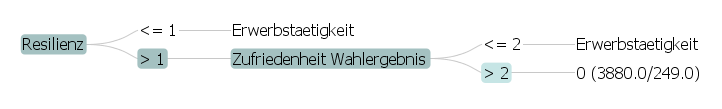
\includegraphics[scale=0.65,angle=0]{fig/treepath}
\captionsetup{width= 380pt}
\caption{Trees were trained using either sci-kit learn or WEKA explorer to identify preprocessing mistakes. The outer right path of the decision-tree demonstrates the desired behavior of the constructed model. "Resilienz"  and "Zufriedenheit Wahlergebnis" have been used to classify the majority of instances as GESIS. Both attributes have been measured on the same scale or mapped properly. Technically, this means that there was no better way to split the data at that specific node. Either the algorithm did not see any gain in continuing to split or the tree was fully grown first and then pruned back using an out-of sample estimations.}
\end{figure}

Figure 4.1 visualizes a path of the latest J48 tree on the current set of features. The entire tree can be seen in the project repository. For the reasons mentioned in Chapter 2, tree-based algorithms are particularly suitable for quickly capturing incorrectly handled data. A subgroup of all participants is said to be representative of the target population, regarding the particular complexity of the trained model. Model complexity, with respect to the right-most leaf node, gives high confidence to include the subgroup of 249 GBS instances in the MRS. 

These trees not only served as indicators for invalid mappings during development, but also for estimating the fraction of latent positives in the GBS surveys. 

\vspace{0.33cm}
\begin{table}[ht]
    \begin{center}
		\captionsetup{width= 430pt}
            {\footnotesize
            \begin{tabular}{l|cccccccccc}
                \hline \hline
                           &  TP Rate & FP Rate & Precision & Recall & F-Measure & ROC Area & PRC Area & Class \\
                \hline
                      LMT & 0.971 & 0.655 & 0.916 & 0.971 & 0.943 & 0.878 & 0.979 & GESIS\\
                      & 0.345 & 0.029 & 0.619 & 0.345 & 0.443 & 0.878 & 0.519 & GBS\\
                \hline \hline
     J48 & 0.973 & 0.710 & 0.910 & 0.973 & 0.940 & 0.716 & 0.928 & GESIS\\
                      & 0.290 & 0.027 & 0.596 & 0.290 & 0.390 & 0.716 & 0.389 & GBS\\
                		
\end{tabular}}
        \caption{Some descriptive statistics of location and dispersion for 2100 observed swap rates for the period from February 15, 1999 to March 2, 2007. Swap rates measured as 3.12 (instead of 0.0312). See Table \ref{Tab:DescripStatsRawDataDetail} in the appendix for more details.}
\label{Tab:DescripStatsRawData}
\end{center}
\end{table}

\section{Estimating the Fraction of Representatives}

In \cite{claesen2}, Claesen et al. emphasize the relative importance of known negatives compared to known positives. This was reason enough, to train a one-class classifier that estimates the GBS class prior with One-Class SVMs. That is, trying to estimate a function which is positive on GESIS and negative on the complement. The dataset that was used for training contains only all positve instances. In one-class SVM, the support vector model is trained on data that has only one class, which is GESIS. It infered the properties of representative cases and from these properties can predict which GBS participants are unlike the normal examples. Predictions from the One-Class SVM are uncalibrated scores that have not been normalized and therefore can not be compared to models based on different algorithms.

\begin{figure}[ht]
\centering
   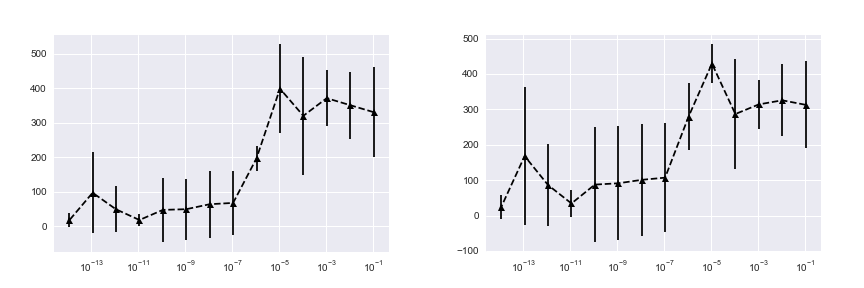
\includegraphics[scale=0.38,angle=0]{fig/occfigure}
\captionsetup{width= 380pt}
\caption{Tuning parameter nu that controls the trade-off between the fraction of non-representative samples and the number of support vectors in one-class SVM. More than 0.73 of GBS (right) are classified as representative with low confidence (high sdt.) for the optimal value \( \nu = 10^5\).}
   \label{fig:Ng1} 
\end{figure}

The two-stage model is conceptually simpler than Algorithm 1, and may in some cases have the greatest practical utility. The main advantage compared to the integrated model is that regularization parameters can be tuned without prior knowledge by cross-validation. Another advantage of the two-stage model is that in the second stage, after the example-specific weights have been derived, virtually any learning mechanism can be employed to produce the final classifier from the weighted training sample. This comes at the cost of only a marginal loss of performance compared to the integrated model. The integrated and two-step logistic regression and exponential models and kernel mean matching perform similarly well.

\section{Maximal Representative Subsample}

A final model is trained with the optimized parameters on the entire data to predict instances of the remaining \(\frac{1}{2}\).

\begin{figure}[ht]
\centering
   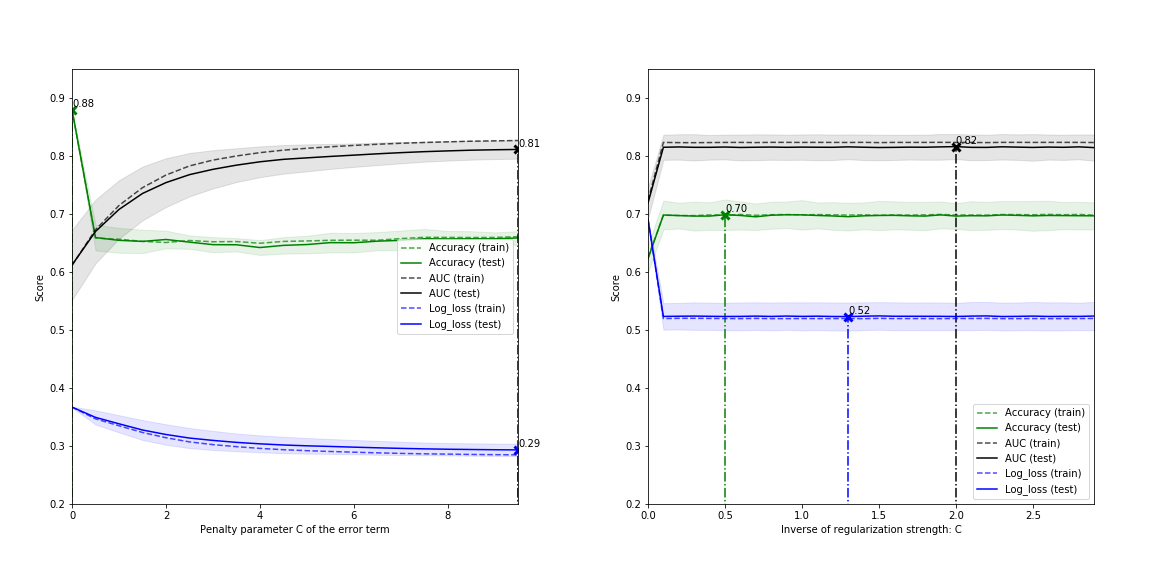
\includegraphics[scale=0.38,angle=0]{fig/gridfigure}
\captionsetup{width= 400pt}
\caption{GridSearchCV: Gridsearch using repeated 10-fold stratified cross-validation on \(\frac{1}{2}\) of the data to evaluate multiple scorers simultaneously. The baselines are 0.89 for accuracy, 0.82 for AUC/AUROC and 0.29 for logarithmic loss. The baselines outperform the trained models on the given metrics, due to the high imbalance in the data.}
   \label{fig:Ng1} 
\end{figure}

\begin{figure}[ht]
\centering
   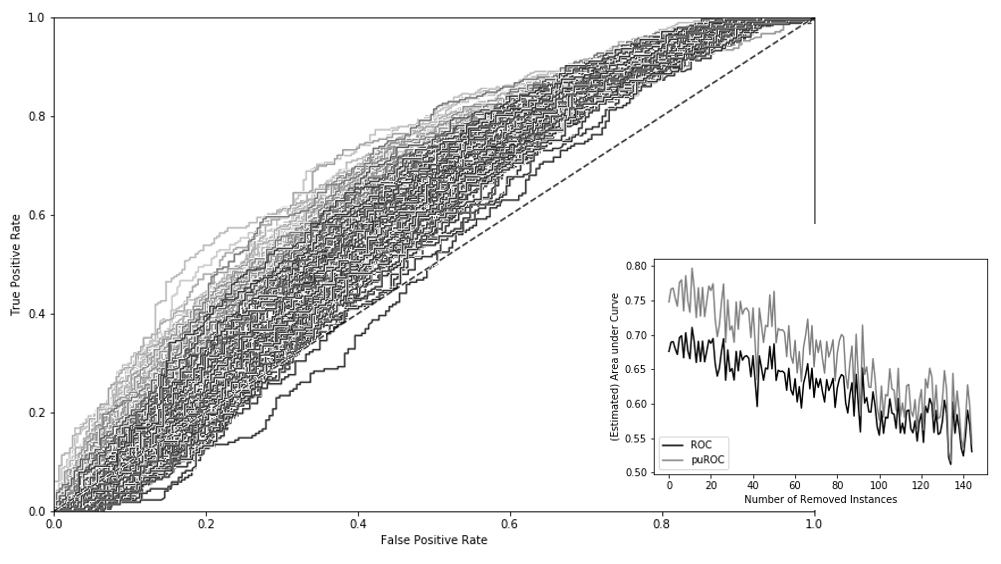
\includegraphics[scale=0.40,angle=0]{fig/res}
\captionsetup{width= 360pt}
\caption{ROC and puROC evaluation for PU learning with Random Forests as base models \cite{breiman2}. An AUROC of approximately \(\frac{1}{2}\) implies that there is no more evidence for covariate shift.}
   \label{fig:Ng1} 
\end{figure}

\begin{figure}[ht]
\centering
\begin{subfigure}[b]{0.8\textwidth}
   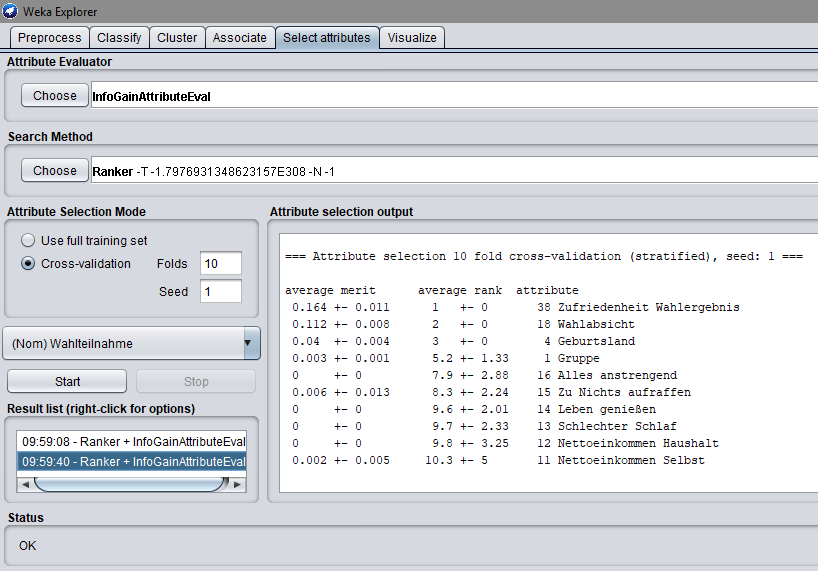
\includegraphics[scale=0.55,angle=0]{fig/weka_gbs}
   \label{fig:Ng1} 
\end{subfigure}
\begin{subfigure}[b]{0.8\textwidth}
\vspace{0.55cm}
   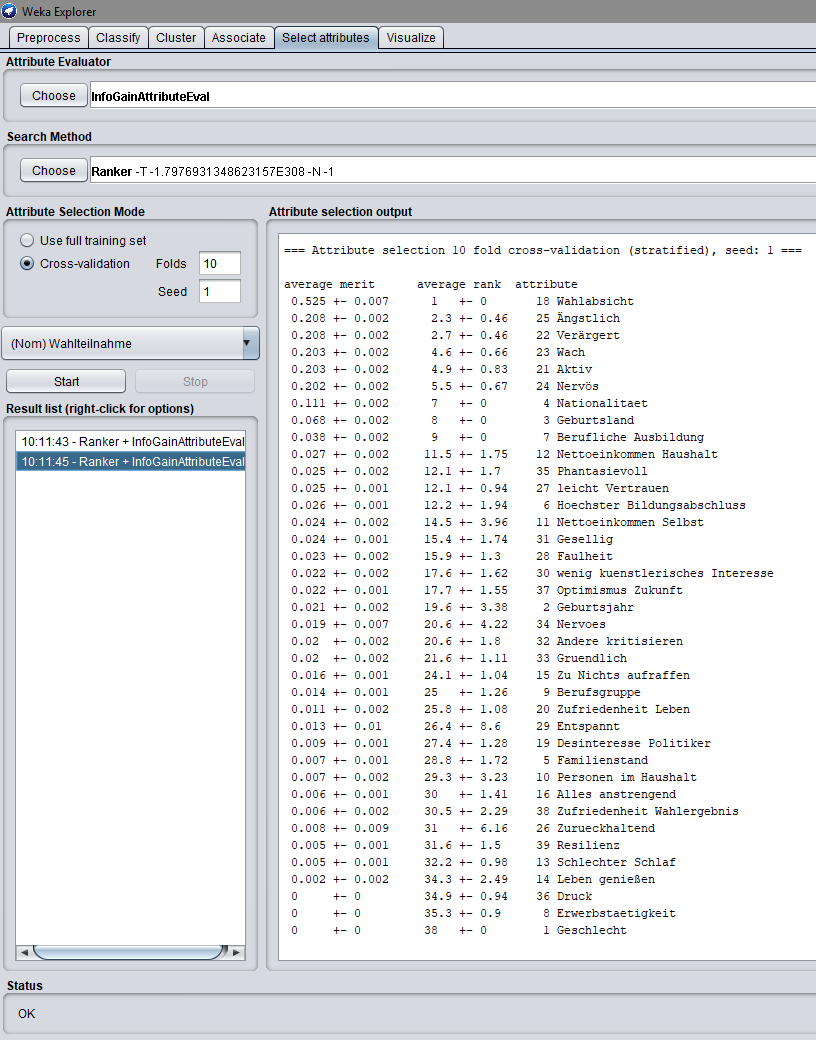
\includegraphics[scale=0.55,angle=0]{fig/weka_gesis}
   \label{fig:Ng2}
\end{subfigure}
\vspace{0.35cm}
\captionsetup{width= 400pt}
\caption{Feature importance in GBS (n=579) and GBS MRS (n=280) for classification of political participation "Wahlteilnahme". In modelling a political participation process, algorithms approximate the likelihood of a person going to vote on election day. Ideally, for every instance with unknown political interest and willingness to participate, there is enough data of people of similiar demographics, socioeconomics and psychological traits to generalize from.}
\end{figure}